%; whizzy chapter
% -initex iniptex -latex platex -format platex -bibtex jbibtex -fmt fmt
% 以上 whizzytex を使用する場合の設定。

%     Kansai Debian Meeting resources
%     Copyright (C) 2007 Takaya Yamashita
%     Thank you for Tokyo Debian Meeting resources

%     This program is free software; you can redistribute it and/or modify
%     it under the terms of the GNU General Public License as published by
%     the Free Software Foundation; either version 2 of the License, or
%     (at your option) any later version.

%     This program is distributed in the hope that it will be useful,
%     but WITHOUT ANY WARRANTY; without even the implied warranty of
%     MERCHANTABILITY or FITNESS FOR A PARTICULAR PURPOSE.  See the
%     GNU General Public License for more details.

%     You should have received a copy of the GNU General Public License
%     along with this program; if not, write to the Free Software
%     Foundation, Inc., 51 Franklin St, Fifth Floor, Boston, MA  02110-1301 USA

%  preview (shell-command (concat "evince " (replace-regexp-in-string "tex$" "pdf"(buffer-file-name)) "&"))
% 画像ファイルを処理するためにはebbを利用してboundingboxを作成。
%(shell-command "cd image200708; ebb *.png")

%%ここからヘッダ開始。

\documentclass[mingoth,a4paper]{jsarticle}
\usepackage{kansaimonthlyreport}
\usepackage[dvips]{xy}
\usepackage{ulem}

% 日付を定義する、毎月変わります。
\newcommand{\debmtgyear}{2014}
\newcommand{\debmtgdate}{27}
\newcommand{\debmtgmonth}{4}
\newcommand{\debmtgnumber}{83}

\def\fixme#1{{\color{red}{#1}}}

\begin{document}

\begin{titlepage}

% 毎月変更する部分、本文の末尾も修正することをわすれずに

 第\debmtgnumber{}回 関西 Debian 勉強会資料

\vspace{2cm}

\begin{center}
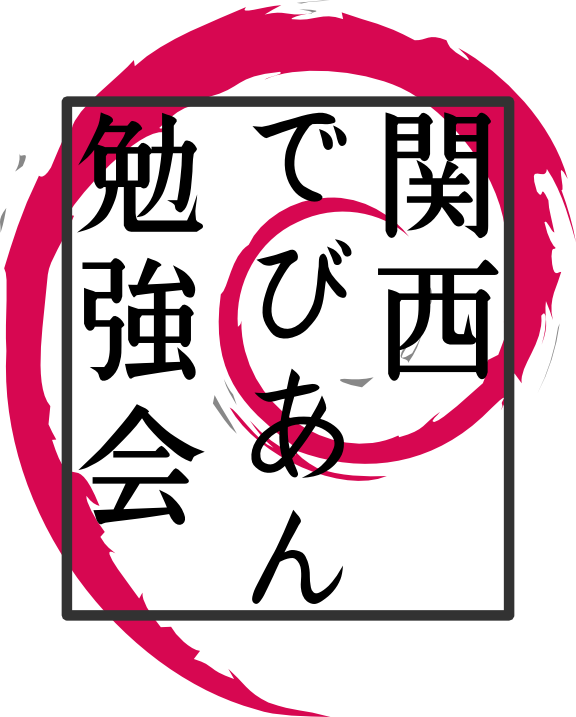
\includegraphics{image200802/kansaidebianlogo.png}
\end{center}

\begin{flushright}
\hfill{}関西 Debian 勉強会担当者 佐々木・倉敷・のがた・かわだ・八津尾 \\
\hfill{}\debmtgyear{}年\debmtgmonth{}月\debmtgdate{}日
\end{flushright}

\thispagestyle{empty}
\end{titlepage}

\dancersection{Introduction}{Debian JP}

\vspace{1em}

 関西Debian勉強会はDebian GNU/Linuxのさまざまなトピック
 (新しいパッケージ、Debian特有の機能の仕組、Debian界隈で起こった出来事、
 などなど)について話し合う会です。

 目的として次の三つを考えています。
 \begin{itemize}
  \item MLや掲示板ではなく、直接顔を合わせる事での情報交換の促進
  \item 定期的に集まれる場所
  \item 資料の作成
 \end{itemize}

 それでは、楽しい一時をお過ごしください。

\newpage

\begin{minipage}[b]{0.2\hsize}
 {\rotatebox{90}{\fontsize{80}{80}
{\gt 関西 Debian 勉強会}}}
\end{minipage}
\begin{minipage}[b]{0.8\hsize}
\hrule
\vspace{2mm}
\hrule
\setcounter{tocdepth}{1}
\tableofcontents
\vspace{2mm}
\hrule
\end{minipage}

\dancersection{最近のDebian関係のイベント報告}{Debian JP}

\subsection{第82回関西Debian勉強会}

82回目の関西Debian勉強会は3月23日(日)に、福島区民センターで行なわれまし
た。

八津尾さんによる「Debian で楽しむ 3D プリンティング」のセッションともく
もくの会でした。

3Dプリンティングを楽しむ秘訣は``折れない心が一番大事''でした。


\subsection{第112回東京エリアDebian勉強会}

112回目の東京エリアDebian勉強会は4月19日(土)に株式会社スクウェア・エニッ
クス 会議室で行なわれました。

前田さんによる「Golang アプリケーション Debian パッケージ」と題した、オー
ケストレーションサポートツールであるSerfを使いたくて、Golangで書かれた
ツールをDebianパッケージにした話のセッションともくもくの会の形式で行な
われました。

これももくもくの会の成果でしょうか、dictoss さんが
「Debian GNU/kFreeBSDでL-02Cを使ってpppする」\footnote{\url{http://pcdennokan.dip.jp/hardware/debian_kfreebsd_ppp/}}
の記事でDebian GNU/kFreeBSDのppp接続の成果を報告されています。

\subsection{Debian Project}

\subsubsection{2014 年 Debian Project Leader}
「Debian Project Leader Election 2014 Results」\footnote{\url{https://lists.debian.org/debian-devel-announce/2014/04/msg00006.html}}
の通り、2014年度の Debian Project Leader に Lucas Nussbaum さんが選出
されました。Lucas さんは 2013 年度に続いて 2 年目の Project Leader と
なります。

おめでとう。Lucas さん。

\subsubsection{Code of conduct}
先月に触れたように Debian に「Code of Conduct(利用上の注意)」を取り入
れようという動きですが、GR(General Resolution:一般決議)に入りました。
「GR: Code of conduct: First call for votes」\footnote{\url{{https://lists.debian.org/debian-devel-announce/2014/04/msg00004.html}}}

\subsubsection{Long term support for Debian 6.0 Announced}

Debian GNU/Linux 6.0 ``squeeze''の長期サポートがアナウンスされました。
\footnote{\url{https://lists.debian.org/debian-announce/2014/msg00002.html}}

i386とamd64アーキテクチャだけが2016年2月までセキュリティサポートを受け
られることになりました。ただし、一部のWeb関連のパッケージは対象外です。

\dancersection{事前課題}{Debian JP}

今回の課題は以下の通りです。
\begin{screen}
  \begin{enumerate}
  \item %
    エミュレータ、仮想化ソフト等を問わず、自分が普段使っているOSと違う
    「OS、もしくはソフト」を使ったことがあるか否か。使用したことのある
    方はその「不満な点を一つ以上上げてください」を教えてください。

  \item %
    もくもくの会で行なう作業、質問などの課題を用意して教えてください。
    (電源とネットワーク(WiMAXなど)はありますが、それ以外の作業に必要な
    環境はご用意ください。)

  \item %
    前回(第82回)の勉強会に参加された方は、前回の作業や課題がその後どう
    なったか結果を教えてください。

  \item %
    LT(ライトニングトーク) 歓迎です。何かお話したい方はタイトルを下さい。
  \end{enumerate}
\end{screen}

参加者の皆さんの解答は以下の通りです:

\begin{prework} { のがたじゅん }
 \begin{enumerate}
  \item Windows。ライセンスが面倒。複数用意しづらい。Linux的作業環境を整えようとすると面倒。
 \end{enumerate}
\end{prework}

\begin{prework}{ takata }

すみません。参加登録するのを忘れていました。

 \begin{enumerate}

  \item 不満な点

        \begin{enumerate}
         \item 仮想エミュレータ全般(kvm, VirtualBox, VMware, etc.)
               環境を立ち上げるのに一手間必要。
               仮想化環境によってはUSBデバイスなどの物理デバイスが使えない場合がある。
         \item chroot環境
               お手軽な反面、仮想化は不十分。
         \item LXC(Linux Containers)
               Debianの場合、設定が少し面倒(Ubuntuに比べて)。
        \end{enumerate}

  \item 第80回勉強会に参加したときの結果について簡単にご報告します。

        \begin{itemize}
         \item 無事、Windows8ノート機(UEFI+GPT)に Debianがインストールできました。
         \item 結局、Windows BootManagerからブートするのはあきらめて、直接Grubから起動することとしました。
        \end{itemize}

 \end{enumerate}

\end{prework}

\begin{prework}{ 木下 }

 \begin{enumerate}
  \item 使用経験:あり
        \begin{itemize}
         \item VMwarePlayer
               \begin{itemize}
                \item ネットワークデバイスの設定がやりにくくなった。
                \item モッサリ感がある。
               \end{itemize}
         \item VMwareServer ※最近は使わなくなったので割愛
         \item VirtualBox
               \begin{itemize}
                \item 設定によるのかもしれませんが、空きメモリを一気に奪われてしまう。
               \end{itemize}
         \item Eucalyptus
               \begin{itemize}
                \item VMではありますが、リソースが物理マシンに依存
                      物理CPU:2、物理MEM:2GBとした場合、VMwarePlayerやVirtualBoxでは上記構成のVMを複数稼働可能ですが(実運用としてはどうかと思う節もありますが・・・)、Eucalyptusは上記構成のVMは1台のみしか稼働できないようです。
                \item インスタンスの記録を手動で行う必要がある
               \end{itemize}
        \end{itemize}

  \item もくもくの会で行なう作業
        \begin{enumerate}

         \item DistCCの調査・研究
         \item Eucalyptus(プライベートクラウドとして)の調査・研究
         \item グリッドコンピューティング関連の調査、研究
               \begin{itemize}
                \item  GlobusToolkitで何ができる?→AndroidOSのクロスコンパイルで使えたら嬉しいかも。
               \end{itemize}
         \item Debian7 on PANDABOARDの調査・研究
               \begin{itemize}
                \item WiFiモジュール(On Board:TI製)の有効化
                \item GPUデバイスドライバの有効化
               \end{itemize}
        \end{enumerate}

  \item 前回(第82回)の勉強会の結果

        \begin{enumerate}
         \item グリッドコンピューティング関連の調査、研究
               \begin{itemize}
                \item GlobusToolkitで何ができる?→AndroidOSのクロスコンパイルで使えたら嬉しいかも。
               \end{itemize}
               \begin{description}
                \item[実績] 保留
               \end{description}
         \item Eucalyptus(プライベートクラウドとして)の調査・研究
               \begin{description}
                \item[実績] インスタンスの起動に成功→起動できなかった原因は、KVMが動作に必要な物理マシンのBIOS設定に誤りがあった。
                \item[課題] 現状、インスタンスを終了させると、今までの結果をすべて忘れてしまうので、インスタンスの記録が必要ですが、現在記録はできるようになりましたが、記録したインスタンスでの起動に失敗してしまう。
               \end{description}
         \item Debian7 on PANDABOARDの調査・研究
               \begin{itemize}
                \item WiFiモジュール(On Board:TI製)の有効化
                \item GPUデバイスドライバの有効化
               \end{itemize}
               \begin{description}
                \item[実績] 保留
               \end{description}
        \end{enumerate}
 \end{enumerate}

\end{prework}

\begin{prework}{ 山城の国の住人 久保博 }

 \begin{enumerate}
  \item あります。
        \begin{description}
         \item[Windows 7] 自分が普段使っている OS になりりつつあること。
         \item[Windows XP] セキュリティ修正がリリースされなくなったこと。
         \item[iOS] 操作するのにキーボードがないこと。
         \item[Android] おなじくキーボードがないこと。
         \item[その他組込機器] 自分ではどうしようもないこと
        \end{description}

  \item Xen のお勉強。 望むらくは xl コマンドで domU を作って起動したい。

  \item 前回は fcm2 のbug \# 647440 の修正バッチを bug 報告に対して投げましたが、なしのつぶてです。
 \end{enumerate}

\end{prework}

\begin{prework}{ yyatsuo }

 \begin{enumerate}
  \item %
       \begin{description}
        \item[組込のリアルタイムOS] μITRON系、VxWorks等
        \item[不満] OSそのものに不満はありません
       \end{description}

       \begin{description}
        \item[NW機器のOS] IOS、ScreenOS等
        \item[不満] 微妙にUnix系のコマンドが使えたり使えなかったりする
       \end{description}

  \item %
       \begin{itemize}
        \item fcitx-skk のパッケージ修正
        \item kernel-handbook の日本語訳の品質向上
       \end{itemize}

  \item %
       \begin{itemize}
        \item fcitx-skk のパッケージング
        \item RFS して岩松さんにスポンサーになってもらった
       \end{itemize}
 \end{enumerate}

\end{prework}

\begin{prework}{ 川江 }

 \begin{enumerate}
  \item ここ、2年ほどXenを使ってました。Xenは準仮想化がデフォルトなので、Widowsなどの仕様の違うOSを使えないのが不満です。
  \item HTMの仕様を調べてみる
  \item spiceでの接続には成功しました。実演する予定です。
 \end{enumerate}

\end{prework}

\begin{prework}{ lurdan }

 \begin{enumerate}
  \item あります。vagrant いいですね。proxmox イケてますね。
  \item webwml-sync の検討をします
  \item python-social-auth は RFS 済み
 \end{enumerate}

\end{prework}

\begin{prework}{ Hiroyuki Nagata }

 \begin{itemize}
  \item 自作の2ちゃんブラウザ、JaneCloneをパッケージとしてDebianに提出する方法など聞く
  \item JaneCloneを久しぶりにDebianでビルドしてパッケージを作る
  \item o2onの移植作業を進める
 \end{itemize}

 ノートパソコンについてはMacしか持っていないため、VM上で作業するつもりです

\end{prework}

\begin{prework}{ Kiwamu Okabe }

 \begin{enumerate}
  \item ATS関連のパッケージ作業
  \item なし
  \item Debianと関連が低いですが、ATS言語 http://jats-ug.metasepi.org/ についてならいくつかしゃべれます
 \end{enumerate}

体調が悪いので、二次会はキャンセルさせてください。。。
よろしくお願いします。
\end{prework}

\begin{prework}{ Hideaki Oose }

 \begin{enumerate}
  \item kfreebsdでjdk1.7の環境構築
  \item kfreebsdでオンボード無線LANによるDHCP接続に成功しました。
  \item ifconfigによるwlandevのcreateと、wpa\_supplicantによるdriverのloadについてLTします。
 \end{enumerate}

\end{prework}

\dancersection{自宅サーバにKVMを導入してみよう}{川江 浩}

\subsection{はじめに}
現在、「クラウド」などで使われている「仮想化技術」ですが、Debianに代表されるdistributionのおかけで、パーソナルベースでも手軽に使えます。

そこで、仮想化技術のKVMを使ってネット関連のサーバ構築や市販のOSをinstallしましたので、システムを構築する際の注意点をレポートします。

また、以下の仕様はパーソナルベースでの運用を前提に構築したものです。仕様を試そうとするときは、必ずデータ等のバックアップをとって自己責任で行ってください。より詳しく知りたい方は専門書を参照してください。

\subsection{仮想化技術}
当初の仮想化はUNIXが動作するサーバやPCアーキテクチャ上で、スーパーバイザ(OS)がハードウェアを管理する形式でした。2000年代になるとIA(Intel Architecture)の処理能力が向上し、IAサーバの仮想マシンモニタが登場しました。

その中のXenは仮想マシンソフトウェアの一つで、OSより1つの下の階層でハイパーバイザというプログラムを管理OSが動かし、仮想化を実現します。

これに対してKVM(Kernel-based Virtual Machine)も同じくハイパーバイザですが、CPUの仮想化支援機能を利用して、機械全体をエミュレーションするシステムエミュレーションのQEMUを高速化し、仮想マシンのOSをアプリケーションとして動かします。


\subsubsection{仮想化の実行モデル}
仮想化の実行モデルとして、準仮想化と完全仮想化の2つがあります。
\begin{itemize}
\item 準仮想化(ParaVirtualization)\\
準仮想化はハードウェアをエミュレートする代わりに、仮想マシン用のハードウェアを使用します。このハードウェアは操作をするためにハイパーバイザコールを呼び出します。ハイパーバイザコールは仮想マシン環境に対応し、ゲストOSは仮想ハードウェア用に修正する必要があります。

\item 完全仮想化(FullVirtualization)\\
完全仮想化機能にはBibary Translationという手法や、CPUの仮想化支援機能を利用した手法があり、デフォルトのOSをそのままで動作させることができます。
\end{itemize}

今回は、qemu-kvmを取り上げましたので以下、仮想化支援を前提にします。
\subsubsection{仮想化支援機能}
CPUで仮想化支援機能は、Intel-VTやAMD-Vなどで、カーネルモードとユーザモード以外にもう一つゲストモードを追加しています。使っているパソコンのハードウェアが仮想化支援機能を利用できるかは、Intel VT-x/d、AMD-Vをサポートしているかによります。

Intelではvmxを
\begin{commandline}
$ grep vmx /proc/cpuinfo
flags   : fpu vme de pse tsc msr pae mce cx8 apic sep mtrr pge mca cmov
 pat pse36 clflush dts acpi mmx fxsr sse sse2 ss ht tm pbe syscall nx lm
 constant_tsc arch_perfmon pebs bts rep_good nopl aperfmperf pni dtes64
 monitor ds_cpl vmx smx est tm2 ssse3 cx16 xtpr pdcm sse4_1 xsave
 lahf_lm dtherm tpr_shadow vnmi flexprioriy
\end{commandline}

AMDではsvmを確認します。
\begin{commandline}
$ grep svm /proc/cpuinfo
flags   : fpu vme de pse tsc msr pae mce cx8 apic sep mtrr pge mca cmov
 pat pse36 clflush mmx fxsr sse sse2 ht syscall nx mmxext fxsr_opt
 pdpe1gb rdtscp lm constant_tsc rep_good nopl nonstop_tsc extd_apicid
 aperfmperf pni pclmulqdq monitor ssse3 fma cx16 sse4_1 sse4_2 popcnt
 aes xsave avx f16c lahf_lm cmp_legacy svm extapic cr8_legacy abm sse4a
 misalignsse 3dnowprefetch osvw ibs xop skinit wdt lwp fma4 nodeid_msr
 tbm topoext perfctr_core arat cpb hw_pstate npt lbrv svm_lock nrip_save
 tsc_scale vmcb_clean flushbyasid decodeassists pausefilter pfthreshold
\end{commandline}

%\clearpage

\subsection{KVMの導入}
次に、qemu-kvmをinstallします。
\begin{commandline}
# apt-get install qemu-kvm
# apt-get install libvirt-bin
\end{commandline}
同時に、GUIのvirt-managerを使った方が仮想マシンの作成、実行、管理が簡単なので、installします。
\begin{commandline}
# apt-get install virt-manager
\end{commandline}
installが終ったら、PCを再起動して、libvirtコマンドを実行するユーザをlibvirtグループのメンバーにしておきます。
\begin{commandline}
# adduser <user> libvirt
\end{commandline}
また、qemu-kvm自体はカネールの機能で、packageで導入する場合はカーネルモジュールとして動作します。

Intel VTの場合
\begin{commandline}
$ lsmod | grep kvm
kvm_intel             121968  0
kvm                   287749  1 kvm_intel
\end{commandline}
AMD-Vの場合
\begin{commandline}
$ lsmod | grep kvm
kvm_amd                47218  10
kvm                   287749  1 kvm_amd
\end{commandline}
\clearpage

\subsubsection{qemu-kvmの仮想ネットワーク}
次に、仮想ネットワークの構成ですが、qemu-kvmの仮想ネットワークはdefaultでnatを使うようになっています。ただし、ネット関連のサーバを構築する場合、サーバを「外部」に公開する必要があります。そこでvirt-managerを使って、仮想ネットワークを接続する仮想bridgeを作成します。
この場合のネットワークインターフェイスはQEMUでエミュレートされ、TAPデバイスを作成して単純に入出力を接続する「tap」を作ります。このtapは擬似的なEthrenetデバイスでLinuxカーネルの機能です。
また、この仮想的なEthrenetデバイスを、同じくLinuxのカネールの機能である仮想bridgeで接続するこで、VMは実デバイスやほかのVMと接続することができます。

%図形の挿入
\begin{figure*}[!h]
\centering
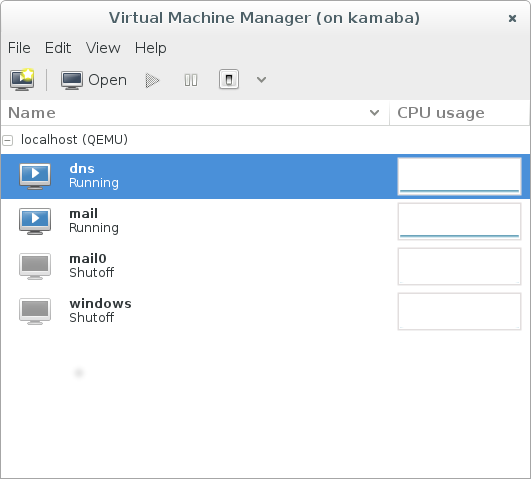
\includegraphics{image201404/virt-manager.png}
\caption{virt-managerの図}
\end{figure*}

\subsubsection{仮想bridgeの作成}
次に、仮想bridgeを作成します。これは、ソフトウェアで802.1d Ethernetブリッジを実装しています。
手順としては、
\begin{enumerate}
\item br0を作成
\item eth0を初期化、br0に接続
\item VMの仮想NICに対応するインターフェイスをbr0に接続
\end{enumerate}

具体的には、virt-managerを立ち上げ「Connection Details」で、「NetworkInterfaces」の「Configure network interface」で「Bridge」を選択し、仮想bridgeにするデバイスを選択してIPアドレス(IPv4)をふります。

%図形の挿入
\begin{figure*}[!b]
\centering
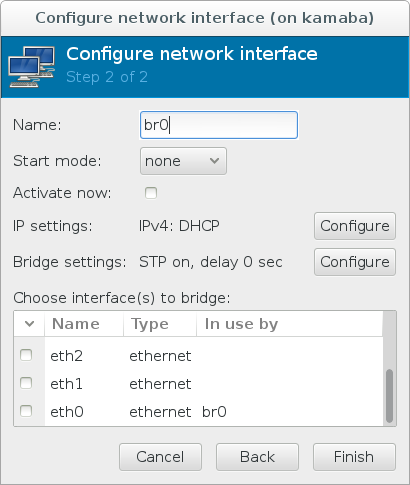
\includegraphics{image201404/bridge2.png}
\caption{bridge設定の詳細の図}
\end{figure*}
\clearpage

後は、VMを作成するときにネットワークで「bridge」を選択すればいいだけです。
イメージとしては以下の「図」のようになります。

ここでeth0は「bridge」として外部につながります。また、セキュリティの関係からeth1は別「segment」にし、eth0から通信を遮断します。このeth1ではSSHなどを使用し、virt-managerで各VMを管理します。そしてeth2はeht0と同じ「segment」にして、後述のSpice専用とします。

\begin{figure*}[!h]
\centering
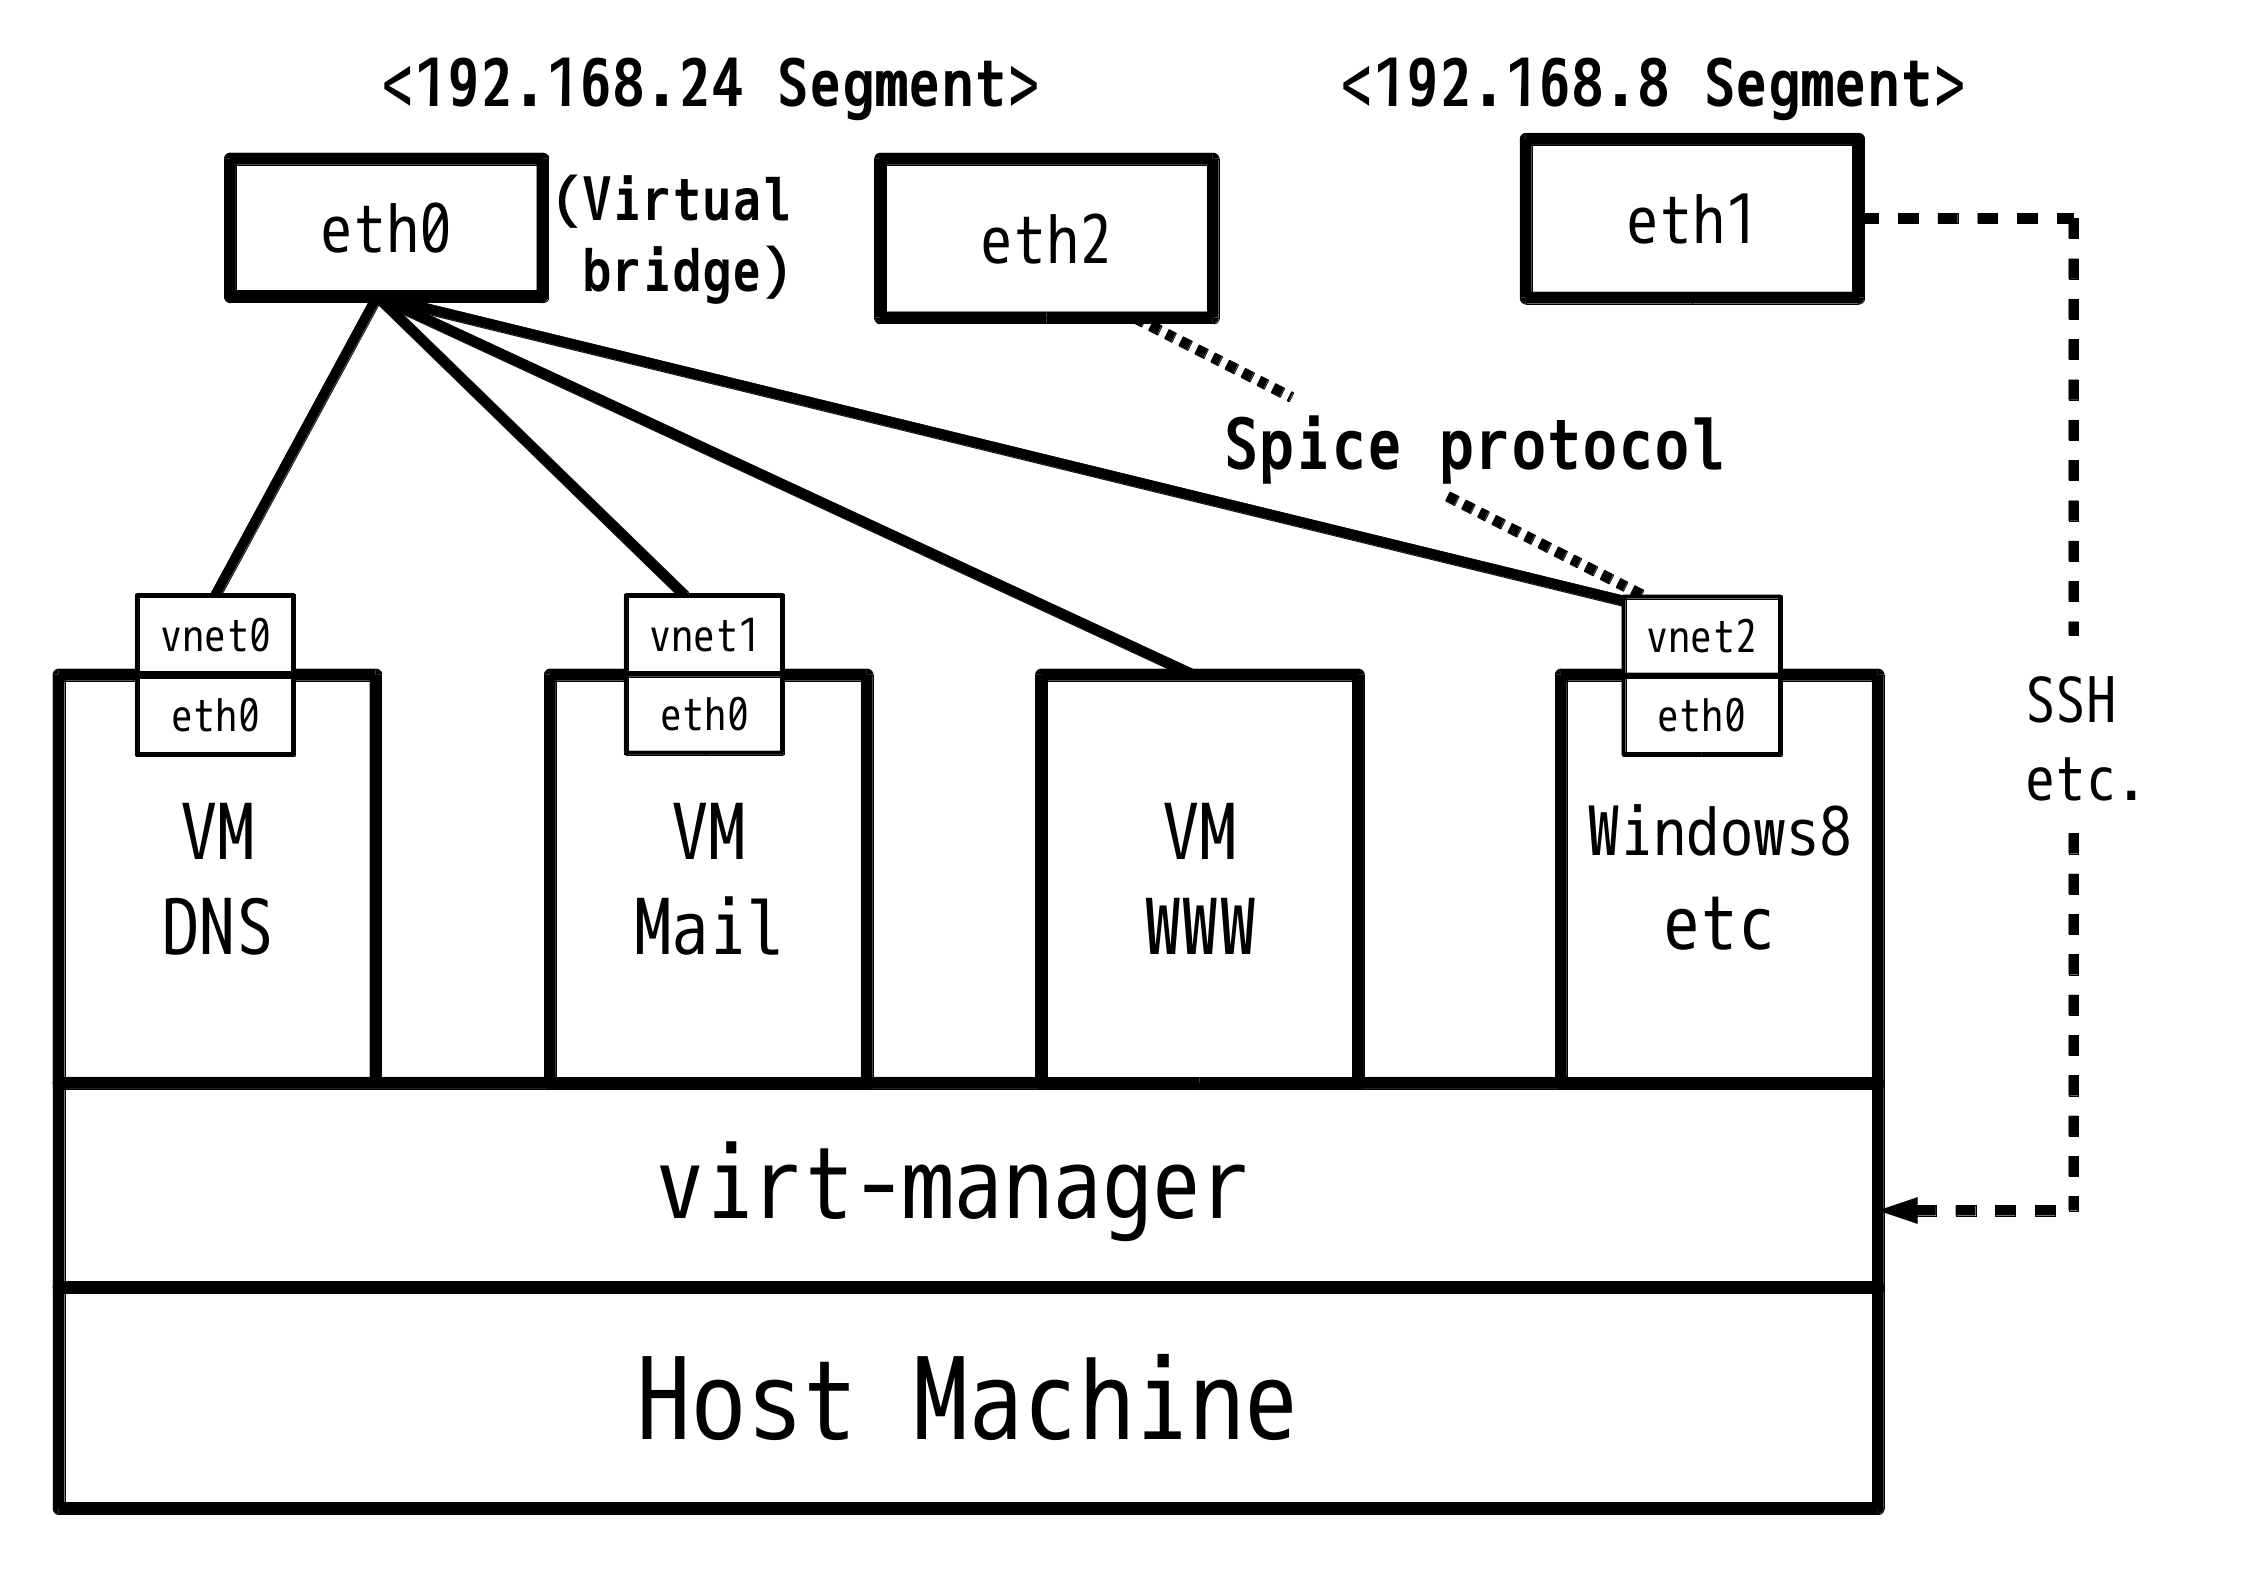
\includegraphics[scale=0.3]{image201404/kvmnetwork3.png}
\caption{ネットワーク構成の図}
\end{figure*}

\subsubsection{Virtual Machineの作成}
次に、virt-managerでVMを作成します。virt-managerはGUIツールのウィザードで、VMの作成時には、物理マシン用のインストールディスク(市販OS)やISOイメージを使いVMを作成します。また、実マシンのリソース内であれば容易にVMの「拡張」ができます。
%Hands onによるインストール

\clearpage

\subsection{各種インターネット関連のサーバの作成}
VMの作成ができたら、各サーバを作成します。まず、DNSの作成にはbind9パッケージをインストールします。
%具体的にwww.kinsen.gr.jpというホスト名に対応するIPアドレスを(再帰)検索する場合、まず、jpドメインのIPアドレスを問い合わせる必要があります。そのために、ルートサーバでjpドメインのIPアドレスを検索し、jpサーバに接続します。同様に、jpに属するgrドメインのIPアドレスを検索し、さらにはgrドメインに属するkinsenそしてwwwと順次、各IPアドレスを検索し、各サーバに接続していきます。そして最終的に、www.kinsen.gr.jpのIPアドレスが203.141.158.41である事がわかります。
\begin{commandline}
# apt-get install bind9
# apt-get install bind9utils
\end{commandline}
DNSの設定ですがNTTの回線の関係上、1個の「グローバル」IPアドレスしか使えなかったので、複数のローカルIPアドレスで各サーバ(クライアント)にIPアドレスを振ります。そこで、acl(Access Control List)でIPアドレスとネットワークを指定し、aclにマッチするクライアントと、その他のクライアントごとに別々ゾーンを提供します。これを利用し、1台のサーバで内部用(aclにマッチする)と外部用(aclにマッチしない)のDNSを構築します。具体的には、
\begin{enumerate}
\item aclで、アドレスマッチリストを設定。
\item クライアント(各サーバ)をIPによって指定し、クライアント毎の振る舞いを作成。
\item viewステートメントで、内部クライアント、外部クライアントに別々のzoneファイルを参照させる。
\end{enumerate}
Mailserverには、Postfix(MTA Mail Transfer Agent)、Dovecot(MDA Mail Delivery Agent)を使います。
\begin{commandline}
# apt-get install postfix
# apt-get install dovecot
\end{commandline}
まず、Postfixについては、saslの認証機構を使ってユーザの認証(SMPT-AUTH)を行い、ユーザ認証で用いるパスワード(平文)をTLSで暗号化します。そして、メール送信のために認証機能のついたサブミッションポートを使用するための設定をします。

devecotはIMAP(Internet Message Access Protocol)プロトコルを使いメールサーバのメールにアクセス、操作、オフラインとオンラインの双方で利用できます。また、Mailサーバの構成については、
\begin{enumerate}
\item 受信したメールをMailディレクトリで扱うように設定
\item imapcopyを使って、旧メールサーバよりメールデータの転送
\item ウィルス対策には、clamtkをインストール
\end{enumerate}

\subsection{サーバの運用・管理}
サーバーの運用・管理は、リモート操作、バックアップ、バッチ処理の実行、トラブルの予防・発見のための稼働監視などが必要ですが、個人で運用する自宅サーバなので、VMのクローンとimport、SPICEを取り上げます。

\subsubsection{VMのclone、import}
バックアップは、VMである各サーバのディスクイメージをベースに、cloneを作ります。このclone(ディスクイメージ)はベースとなったVMとまったく同じ「構成」ですが、virt-managerを使ってMACアドレスの変更ができます。また、イメージをKVMが走っている別のマシンにimportできます。また、各種サーバの構築の際は「ベースのVM」を作成し、クローンを作って『カタマイズ』するなどの使い方ができます。

\subsubsection{SPICE}
リモート操作にはSPICEを使います。SPICE(Simple Protocol for Independent Computing Environment)は、仮想化環境上に構築したデスクトップ環境にリモートから接続するという仮想デスクトップ環境(VDI)です。特徴は、オープンソースの画面転送プロトコルで、高画質なビデオ転送と高音質な双方向音声転送ができることです。

次に、spiceクライアントをインストールし、ターミナルから接続します。
\begin{commandline}
# apt-get install spice-client
\end{commandline}
続いて、qemu-kvmのVMに接続します。
\begin{commandline}
$ spicec -h noren.kinsen.gr.jp -p 590X -w *********
\end{commandline}
「-h」はホスト名、「-p」はポート番号、「-w」はログインするためのパスワードです。

\subsection{まとめ}
まとめとして、自分の自宅サーバはこの間、2年ほど「Xen」で運用していました。Xenはqemu-kvmと同じハイパーバイザなのですが、仮想化のモデルが準仮想化なので、サーバに多くのリソースは必要ありません(メールサーバ、DNSともども384MBで運用しました)。ただ、リソースが十分に用意できるのであれば、OSをdefaultで使える点や、virt-managerなどのツール、「高速」「高機能」のSPICEが使用できるなどの利点がqemu-kvmにはあります。

今後の予定としては、WWWサーバでは「HTML5」を使ったサイトの構築や、IPv6への対応(ただし、パーソナルレベルでGlobal Routing Prefixが /48-/64bit内であることが前提)、さらなる『異種』のOSのVM化をしたいと思っています。


\dancersection{Notmuch Mail}{David Bremner}

Originally inspired by the sup mail user agent (MUA), notmuch is a GPL3+
set of tools for for dealing with your mail (stored in Maildirs or
similar) via searching and tagging. On top of the C bindings and a
scriptable command line interface, the project directly supports user
interfaces based on Emacs and VIM as well as integration with Mutt. We
also support python, ruby, and go bindings. Other projects based on
notmuch include curses based frontends written in python and Mercury, a
fork of mutt using notmuch as a the backend, a web interface, and a
virtual maildir filesystem.  In this lightning talk I'll give a tour of
the notmuch "ecosystem", concentrating on the Emacs interface and
command line tool.


\dancersection{もくもくの会}{}

\dancersection{今後の予定}{Debian JP}

\subsection{関西Debian勉強会}

次回、第84回関西Debian勉強会は5月25日(日)に福島区民センターで開催します。

\subsection{東京エリアDebian勉強会}
第113回東京エリアDebian勉強会は5月17日(土)に場所は未定ですが開催予定です。

%
% 冊子にするために、4の倍数にする必要がある。
% そのための調整
\dancersection{メモ}{}
\mbox{}\newpage
%% \mbox{}\newpage
%% \mbox{}\newpage

\printindex
%\cleartooddpage

 \begin{minipage}[b]{0.2\hsize}
  \rotatebox{90}{\fontsize{80}{80} {\gt 関西 Debian 勉強会} }
 \end{minipage}
 \begin{minipage}[b]{0.8\hsize}

 \vspace*{15cm}
 \rule{\hsize}{1mm}
 \vspace{2mm}
 
\includegraphics[width=2cm]{image200502/openlogo-nd.eps}
 \noindent \Large \bfseries{Debian 勉強会資料}\\ \\
 \noindent \normalfont \debmtgyear{}年\debmtgmonth{}月\debmtgdate{}日 \hspace{5mm}  初版第1刷発行\\
 \noindent \normalfont 関西 Debian 勉強会 (編集・印刷・発行)\\
 \rule{\hsize}{1mm}
 \end{minipage}

\end{document}
